\section{Al2O3}
\subsection*{Material ID: mp-bqvqw}
\textbf{Constante Dieléctrica ($\epsilon_{total}$):} 8.81 \\[0.5em]
\begin{table}[h!]
\centering
\begin{tabular}{lcc}
\toprule
\textbf{Métrica} & \textbf{Lámina (Plate)} & \textbf{Cilindros (Rod)} \\
\midrule
Bandgaps ($a/\lambda$) & Ninguno & Ninguno \\
Resonancias & 36 & 36 \\
\bottomrule
\end{tabular}
\end{table}
\begin{figure}[H]
\centering
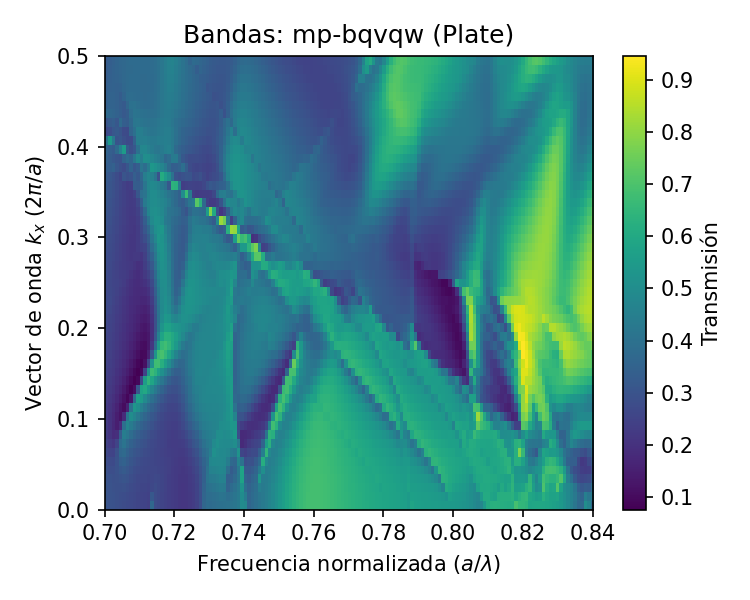
\includegraphics[width=0.48\textwidth]{figures/mp-bqvqw_plate.png}
\hfill
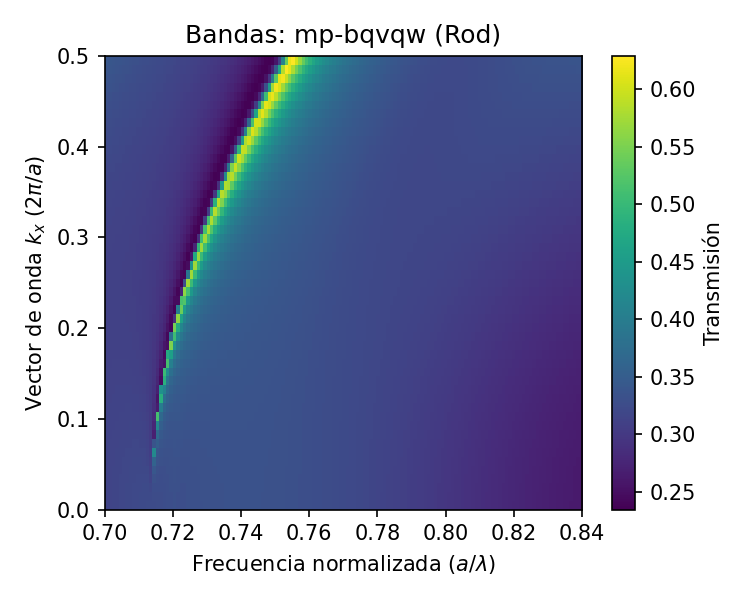
\includegraphics[width=0.48\textwidth]{figures/mp-bqvqw_rod.png}
\caption{Estructuras de bandas fotónicas para mp-bqvqw. Izquierda: Lámina. Derecha: Cilindros.}
\end{figure}
\vspace{1em}
\hrule
\vspace{1em}

\subsection*{Analisis}

De nuevo pude encontrarlo en la misma pagina (que como puede ver resulto supremamente util) \url{https://order.universitywafer.com/default.aspx?cat=Sapphire} de nuevo en forma de placa (y de nuevo eso es una gran noticia pues este resultado es mucho mas interesante). Curiosamente este resulta tener una variación de precio bastante mayor que los otros entonces necesitariamos mirar con mas detalle para decantarnos por esta opcion) en los terminos fisicos se encuentra en condiciones similares a los anteriores. No se encuentran Gaps evidentes ni demasiado grandes que obtener.

\clearpage
